\documentclass{article}

\usepackage[utf8]{inputenc}
\usepackage{tikz}
\usepackage{amsmath}
\usepackage{mathtools}
\usepackage{amsfonts}
\usepackage{amssymb}
\usepackage{sectsty}
\usepackage{xcolor}
\usepackage[paperwidth=180mm, paperheight=290mm, left=10mm, top=10mm, bottom=10mm, right=10mm, margin=10mm]{geometry}
\usepackage{ragged2e}
\usepackage{listings}

\definecolor{def}{RGB}{255, 173, 97}
\definecolor{tit}{RGB}{217, 84, 80}
\definecolor{emp}{RGB}{150, 206, 180}
\definecolor{acc}{RGB}{255, 238, 173}
\definecolor{txt}{RGB}{249, 232, 232}
\definecolor{back}{RGB}{22, 22, 22}

\sectionfont{\color{tit}\fontsize{20.74}{35}\ttfamily}
\subsectionfont{\color{tit}\fontsize{17.28}{17.28}\ttfamily}

\DeclareFontFamily{\encodingdefault}{\ttdefault}{%
  \hyphenchar\font=\defaulthyphenchar
  \fontdimen2\font=0.33333em
  \fontdimen3\font=0.16667em
  \fontdimen4\font=0.11111em
  \fontdimen7\font=0.11111em
}

\newcommand{\R}{\mathbb{R}}
\newcommand{\N}{\mathbb{N}}
\newcommand{\Q}{\mathbb{Q}}
\newcommand{\Z}{\mathbb{Z}}
\newcommand{\C}{\mathbb{C}}
\newcommand{\cont}{\mathfrak{c}}

\geometry{a4paper, textwidth=155mm, textheight=267mm, left=15mm, top=15mm, right=15mm, marginparwidth=0mm}
\setlength\parindent{15pt}

\pagestyle{empty}

\begin{document}\pagecolor{back}\color{txt}\ttfamily
\section*{ZBIORY Z POWTORZENIAMI}
Wezmy piec kulek:
\begin{center}
    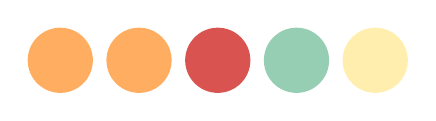
\begin{tikzpicture}
        \filldraw[color=def, fill=def, thick] (0, 0) circle (0.4);
        \filldraw[color=def, fill=def, thick] (1, 0) circle (0.4);
        \filldraw[color=tit, fill=tit, thick] (2, 0) circle (0.4);
        \filldraw[color=emp, fill=emp, thick] (3, 0) circle (0.4);
        \filldraw[color=acc, fill=acc, thick] (4, 0) circle (0.4);
    \end{tikzpicture}
\end{center}
Chcemy policzyc ile jest permutacji piecioelementowego zbioru, w ktorym jeden element powtarza sie dwa razy, ale powtorzenia sie miedzy soba nierozroznialne? Podpiszmy kolejne kule cyframi:
\begin{center}
    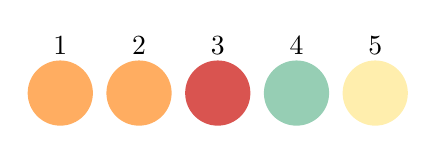
\begin{tikzpicture}
        \node (a) at (0, 0.6) {1};
        \node (b) at (1, 0.6) {2};
        \node (v) at (2, 0.6) {3};
        \node (d) at (3, 0.6) {4};
        \node (e) at (4, 0.6) {5};
        \filldraw[color=def, fill=def, thick] (0, 0) circle (0.4);
        \filldraw[color=def, fill=def, thick] (1, 0) circle (0.4);
        \filldraw[color=tit, fill=tit, thick] (2, 0) circle (0.4);
        \filldraw[color=emp, fill=emp, thick] (3, 0) circle (0.4);
        \filldraw[color=acc, fill=acc, thick] (4, 0) circle (0.4);
    \end{tikzpicture}
\end{center}
Wowczas, rozmiescic je mozemy na $5!$ sposobow. Wiemy jednak, ze dwie czerwone kule sa dla nas nierozroznialne, wiec mozemy je miedzy soba przestawiac dowoli - mamy \color{emp}$\frac{5!}{2!}$ \color{txt}sposobow ustawienia tych kul.\bigskip
\begin{center}
    \color{def}ZBIOR Z POWTORZENIAMI \color{txt}bedziemy zapisywac jako:
    $$A=\{n_1\cdot a_1, n_2\cdot a_2,..., n_k\cdot a_k\},$$
    gdzie $n_1, n_2, ..., n_k$ to powtorzenia elementow odpowiednio $a_1, a_2, ..., a_k$.
\end{center}\bigskip
Zastanowmy sie, na ile jest permutacji zbioru
$$A=\{2\cdot a, 3\cdot b, 4\cdot c\}?$$
Jesli takie same elementy byly rozroznialne, byloby $9!$ permutacji takiego zbioru. Jednak jednakowe elementy sa nierozroznialne, wiec liczba permutacji to:
$${9!\over 2!\cdot3!\cdot4!}$$
\subsection*{DUZA CUKIERNIA}
    Przychodzimy do cukierni, ktora sprzedaje \color{acc}paczki, eklerki, serniki i makowce\color{txt}. Cukiernia jest duza, wiec nie ma ograniczen co do ilosci kazdego produktu. My chcemy kupic 6 ciastek i zastanawiamy sie, \color{emp}na ile sposobow mozemy to zrobic?\color{txt}\smallskip\\
    Rownowaznie mozemy to zapisac jako pytanie \color{emp}ile rozwiazan calkowitych nieujemnych ma rownanie\color{txt}
    $$x_1+x_2+x_3+x_4=6?$$
    \color{acc}Wyobrazmy sobie, ze w naszym tobolku na ciastka mamy 6 przegrodek:
    $$1\quad1\quad1\quad1\quad1\quad1\quad=6$$
    Zakodujemy nasz sposob zakupu wstawiajac w ten ciag 0\color{txt}, czyli 3 paczki, dwie eklerki i jeden sernik to:
    $$1\quad1\quad1^0\quad1\quad1^0\quad1^0\quad$$
    W takim razie liczba sposob na jaki mozemy kupic 6 ciastek to liczba sposobow na jakie mozemy ustawic 3 zera i 6 jedynek:
    $$p={9!\over3!\cdot6!}\bigskip$$
    \begin{center}
        Ze zbioru A zawierajacego \color{def}$m$ roznych elementow \color{txt}mozemy wybrac \color{def}$k$ elementow \color{txt}z powtorzeniami na
        $$\color{emp}{m-1+k\choose k}={(m-1+k)!\over k!\cdot(m-1)!}$$
        sposobow i jest to liczba rozwiazan rownania
        $$x_1+x_2+...+x_m=k$$
        w nieujemnych liczbach calkowitych $x_1, x_2,...,x_m$
    \end{center}
\subsection*{ZASADA WLACZEN I WYLACZEN}
    \begin{center}Dla dwoch zbiorow skonczonych zachodzi:
        $$\color{def}|A\cup B|=|A|+|B|-|A\cap B|$$
        $$|A|+|B|=|(A\setminus B)\cup(A\cap B)|+|B|=|A\setminus B|+|A\cap B|+|B|=|A\cup B|+|A\cap B|$$
    \end{center}
    Ile jest liczb $1\leq n\leq100$ podzielnych przez 2 lub podzielnych przez 3?\smallskip\\
    Liczb podzielnych przez 2 mamy $\lfloor{100\over2}\rfloor=50$, liczb podzielnych przez dwa mamy $\lfloor{100\over 3}\rfloor=33$. Ale w obu tych zbiorach znajduja sie liczby podzielne i przez 2 i przez 3, czyli podzielne przez 6. Musimy wiec odjac jedno ich powtorzenie, czyli $\lfloor{100\over6}\rfloor=16$.\smallskip\\
    Jest $50+33-16=67$ liczb podzielnych przez 2 lub przez 3.\medskip\\
    $$\color{acc}|A\cup B\cup C|=|A|+|B|+|C|-(|A\cap B|+|B\cap C|+|A\cap C|)+|A\cap B\cap C|$$
    \begin{center}
        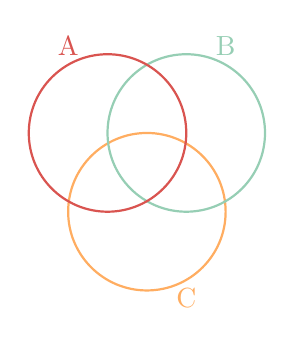
\begin{tikzpicture}
            \node(a) at (1, 2.1) {\color{emp}B};
            \node(b) at (-1, 2.1) {\color{tit}A};
            \node(c) at (0.5, -1.1) {\color{def}C};
            \draw[color=def, thick] (0, 0) circle (1);
            \draw[color=emp, thick] (0.5, 1) circle (1);
            \draw[color=tit, thick] (-0.5, 1) circle (1);
        \end{tikzpicture}
    \end{center}
    \emph{dowod na cwiczeniach}
    \begin{center}
        Dla dowolnych zbiorow skonczonych $A_1, ..., A_n$ zachodzi wzor
        $$|A_1\cup A_2\cup...\cup A_n|=\sum\limits_{i=1}^n|A_i|-\sum\limits_{i<j}|A_i\cap A_j|+\sum\limits_{i<j<k}|A_i\cap A_j\cap A_k|+...+(-1)^{n+1}|A_1\cap A_2\cap...\cap A_n|$$
    \end{center}
    Dowod:\\
    Wezmy dowolny element nalezacy do dowolnego ze zbiorow:
    $$x\in A_1\cup A_2\cup ...\cup A_n.$$
    Niech teraz $k$ bedzie iloscia tych zbiorow, w ktorych $x$ sie pojawia. Zastanawiamy sie teraz, ile razy $x$ bedzie liczony po prawej stronie?
    $$k-{k\choose2}+{k\choose3}+...+(-1)^{k+1}{k\choose k}$$
    $${k\choose1}-{k\choose2}+{k\choose3}+...+(-1)^{k+1}{k\choose k}=1$$
    $$0={k\choose0}+{k\choose1}-{k\choose2}+{k\choose3}+...+(-1)^{k+1}{k\choose k}=(1+(-1))^k=0^k$$
    \emph{bardziej formalnym dowodem jest dowod przez indukcje}
\subsection*{MALA CUKIERNIA}
    \color{acc}Ile jest 11-kombinacji ze zbioru $\{3\cdot a, 4\cdot b, 5\cdot c\}$?\color{txt}\smallskip\\
    Nie pytajmy sie ile wezmiemy do naszego zbioru, a ile zostanie? Tutaj mamy 12 elemntow i zostaje nam zawsze 1 - mozemy wyrzucic $a,b,\texttt{ lub }c$. W takim razie odpowiedz to \color{emp}3\color{txt}.\medskip\\
    \color{acc}Ile jest 10-kombinacji ze zbioru $\{3\cdot a, 4\cdot b, 5\cdot c\}$?\color{txt}\smallskip\\
    Tyle samo, ile jest 2-kombinacji z tego zbioru, czyli ${3-1+2\choose2}={4\choose2}=6$.\medskip\\
    \color{def}PRZYKLAD TYPOWY \color{acc}Ile jest 10-kombinacji ze zbioru $X=\{3\cdot a, 4\cdot b, 5\cdot c, 6\cdot d\}$?\color{txt}\smallskip\\
    Najpierw zastanawiamy sie, co by bylo gdyby to byla duza cukiernia? Wedlug poprzedniego schematu mamy ${13\choose10}$. Teraz musimy pozbyc sie tych kombinacji, ktore sa niemozliwe ze wzgledu na ilosc poszczegolnych elementow. Kombinacjami zlymi sa:\\
    $Z(a)\texttt{ - zle kombinacje, w ktorych }a\texttt{ pojawia sie }\geq 4$\\
    $Z(b)\texttt{ - zle kombinacje, w ktorych }b\texttt{ pojawia sie }\geq 5$\\
    $Z(c)\texttt{ - zle kombinacje, w ktorych }c\texttt{ pojawia sie }\geq 6$\\
    $Z(d)\texttt{ - zle kombinacje, w ktorych }d\texttt{ pojawia sie }\geq 7$\\
    $${13\choose10}-|Z(a)\cup Z(b)\cup Z(c)\cup Z(d)|$$
    Teraz musimy policzyc moc sumy zbiorow zawierajacych zle kombinacje. Do tego potrzebne sa nam moce poszczegolnych zbiorow:\\
    $|Z(a)|={9\choose6}$ czyli liczba 6-kombinacji ze zbioru $D=\{\infty\cdot a, \infty\cdot b, \infty\cdot c, \infty\cdot d\}$, bo moge max 4 razy wybrac $a$, wiec zeby to byla zla kombinacja, na pozostalych miejscach tez musi sie pojawic co najmniej jedno $a$\\
    $|Z(b)|={8\choose5}$, natomiast $|Z(a)\cap Z(b)|=4$.
\end{document}